% !TEX root=../report.tex

\section{Experiments}
\label{sec:experiment}

For this project, we trained our reinforcement learning models on 3 scenarios in the predator prey setting - 1) 1 green agent vs 1 red agent, 2) 2 green agents vs 1 red agent and 3) 1 green agent vs 2 red agents. We did not use any landmarks, as none of the algorithms we employ explicitly model the landmarks in their optimization, i.e., there is no constraint/penalty that prevents agents from attempting to "move through" the landmarks. Each of the 3 scenarios described above were performed with DQN, DDPG and MADDPG agents separately. The number of steps, collisions, average reward and average loss per episode were collected for all experiments. TODO: DQN vs MADDPG  

\subsection{1 Green Agent vs. 1 Red Agent}
\label{sec:experiment:1vs1}

In the 1 green agent vs 1 red agent scenario, we expect our reinforcement learning models to learn that an agent should not go outside the arena. We also expect the number of collisions between both agents to decrease over time as the faster green agent learns to out maneuver the slower red agent.

From Figure~\ref{fig:1vs1}, we observe that the average number of steps (i.e., how long each episode lasts) increases over time for all models, confirming that the agents learn not to go outside the arena. If the rewards for collisions and stepping outside the arena are ignored, then this scenario is zero sum. This is confirmed by the rewards vs episodes plots which suggest that the sum of the average rewards for both agents is close to zero for all models. For the DQN agents, we notice that the average number of collisions decreases over episodes. However, the collisions and average loss plots suggest that unlike the DQN agents, the DDPG and MADDPG agents have not yet formulated stable policies.

\begin{figure}[t]
  \vspace*{-2cm}
  \begin{subfigure}[t]{\figscale\linewidth}
    \hspace*{-2.75cm}
    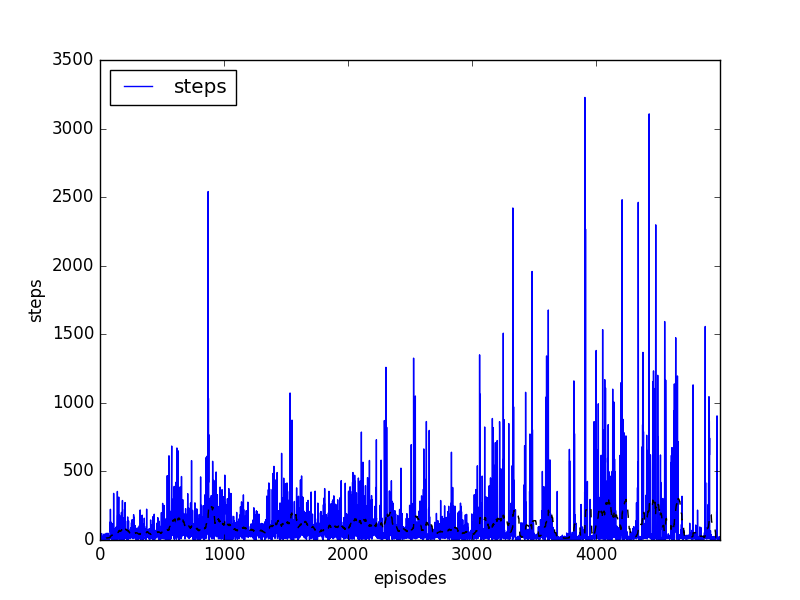
\includegraphics[width=1.5\textwidth]
    {../results/dqn_1vs1/steps.png}
    \label{fig:dqn-1vs1-steps}
  \end{subfigure}
  ~
  \begin{subfigure}[t]{\figscale\linewidth}
    \hspace*{-1.4cm}
    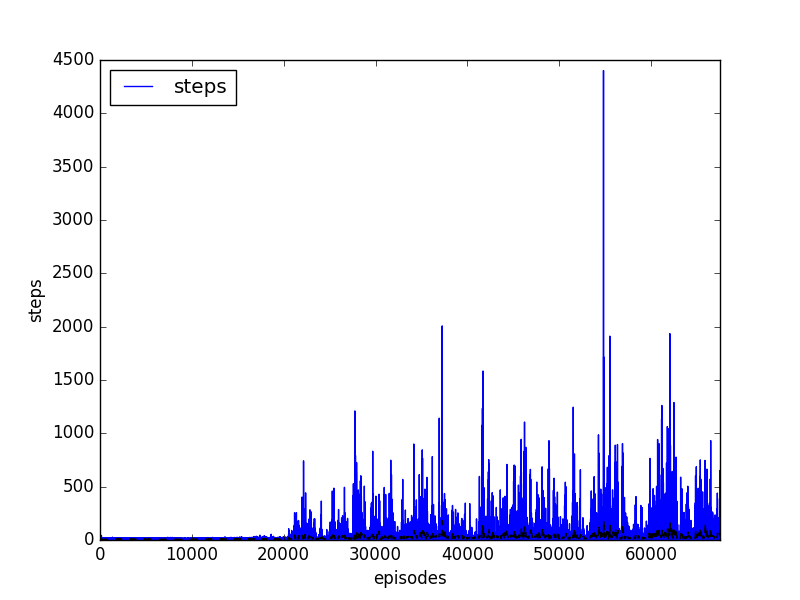
\includegraphics[width=1.5\textwidth]
    {../results/ddpg_1vs1/steps.png}
    \label{fig:ddpg-1vs1-steps}
  \end{subfigure}
  ~
  \begin{subfigure}[t]{\figscale\linewidth}
    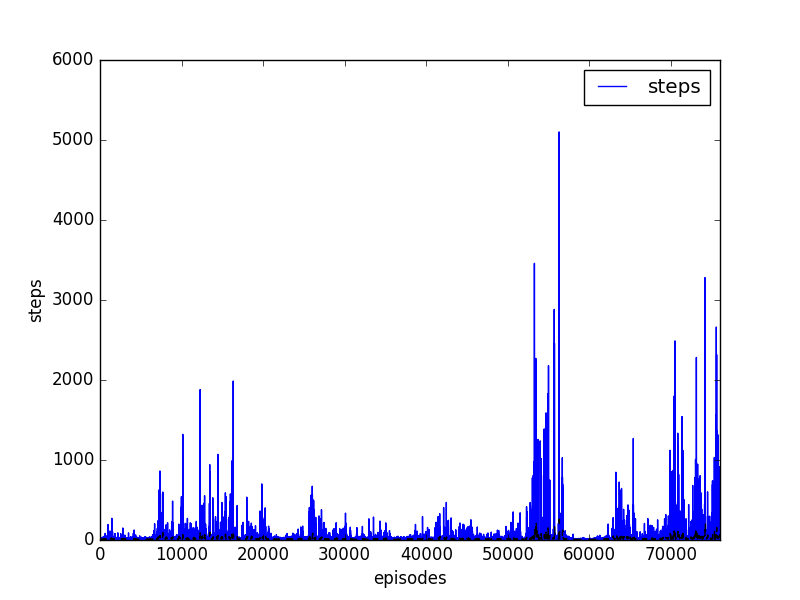
\includegraphics[width=1.5\textwidth]
    {../results/maddpg_1vs1/steps.png}
    \label{fig:maddpg-1vs1-steps}
  \end{subfigure}

  \vspace{-0.5cm}
  \begin{subfigure}[t]{\figscale\linewidth}
    \hspace*{-2.75cm}
    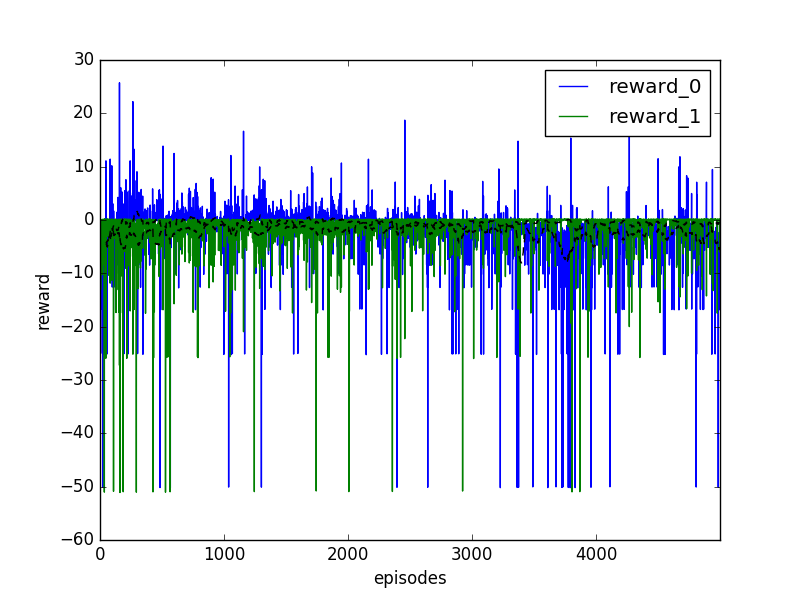
\includegraphics[width=1.5\textwidth]
    {../results/dqn_1vs1/reward.png}
    \label{fig:dqn-1vs1-reward}
  \end{subfigure}
  ~
  \begin{subfigure}[t]{\figscale\linewidth}
    \hspace*{-1.4cm}
    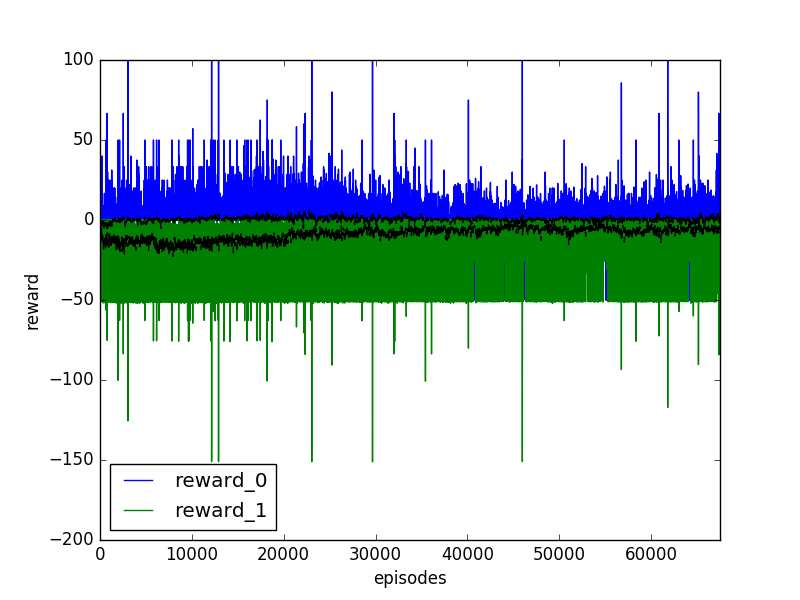
\includegraphics[width=1.5\textwidth]
    {../results/ddpg_1vs1/reward.png}
    \label{fig:ddpg-1vs1-reward}
  \end{subfigure}
  ~
  \begin{subfigure}[t]{\figscale\linewidth}
    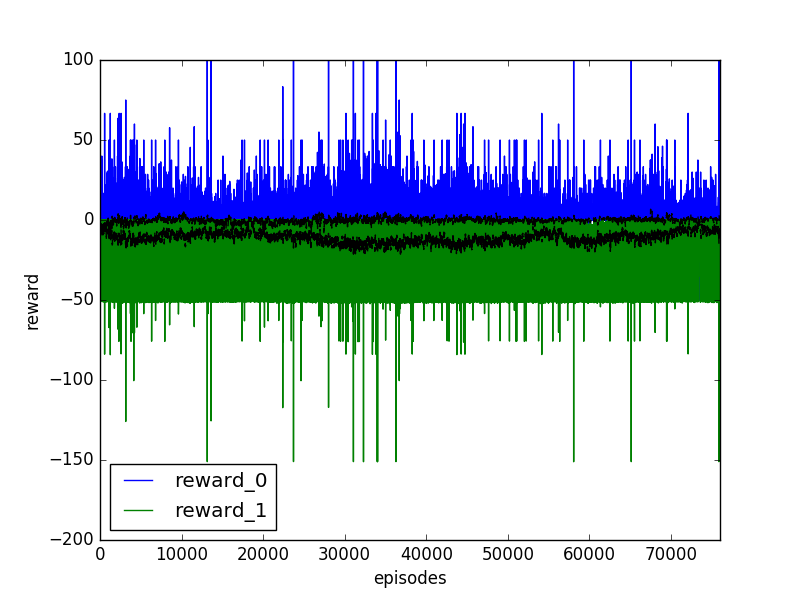
\includegraphics[width=1.5\textwidth]
    {../results/maddpg_1vs1/reward.png}
    \label{fig:maddpg-1vs1-reward}
  \end{subfigure}

  \vspace{-0.5cm}
  \begin{subfigure}[t]{\figscale\linewidth}
    \hspace*{-2.75cm}
    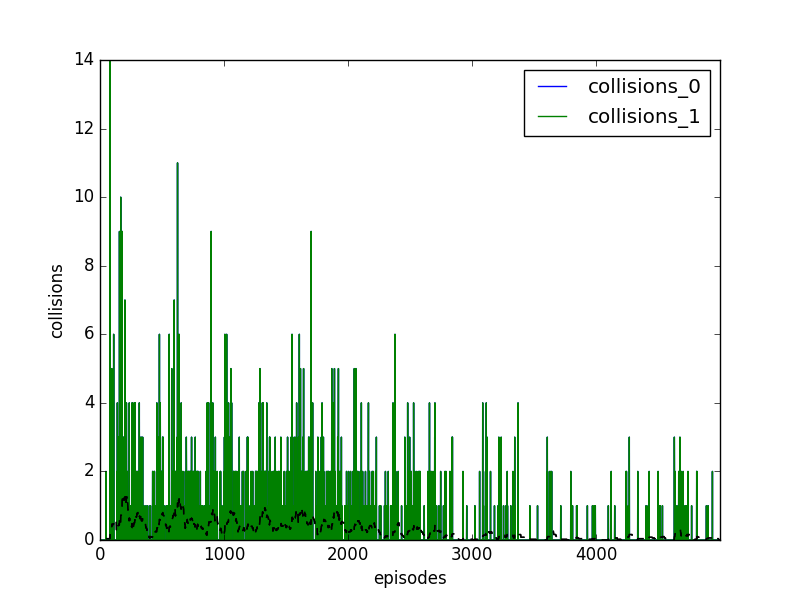
\includegraphics[width=1.5\textwidth]
    {../results/dqn_1vs1/collisions.png}
    \label{fig:dqn-1vs1-collisions}
  \end{subfigure}
  ~
  \begin{subfigure}[t]{\figscale\linewidth}
    \hspace*{-1.4cm}
    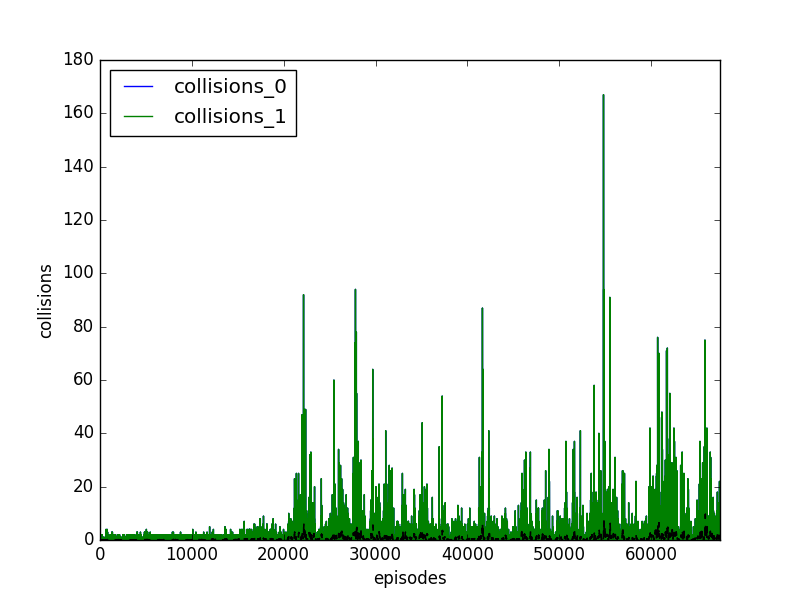
\includegraphics[width=1.5\textwidth]
    {../results/ddpg_1vs1/collisions.png}
    \label{fig:ddpg-1vs1-collisions}
  \end{subfigure}
  ~
  \begin{subfigure}[t]{\figscale\linewidth}
    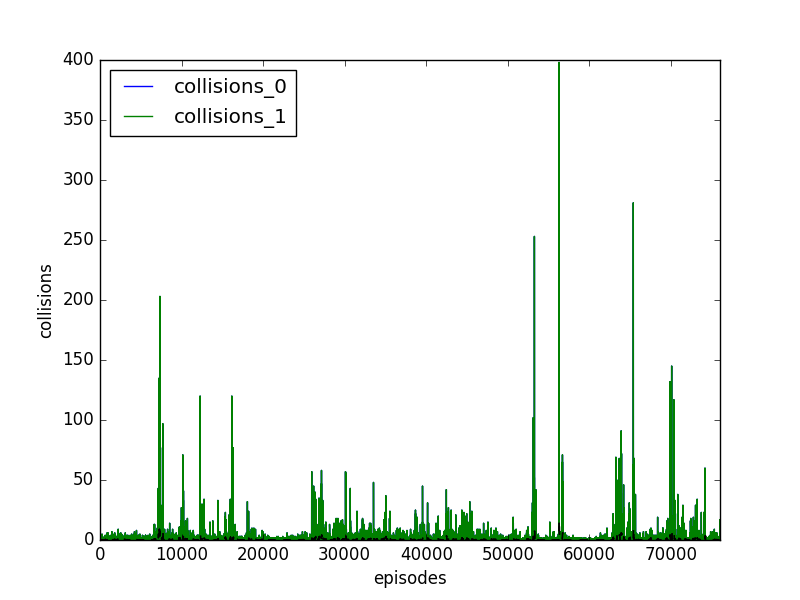
\includegraphics[width=1.5\textwidth]
    {../results/maddpg_1vs1/collisions.png}
    \label{fig:maddpg-1vs1-collisions}
  \end{subfigure}

  \vspace{-0.5cm}
  \begin{subfigure}[t]{\figscale\linewidth}
    \hspace*{-2.75cm}
    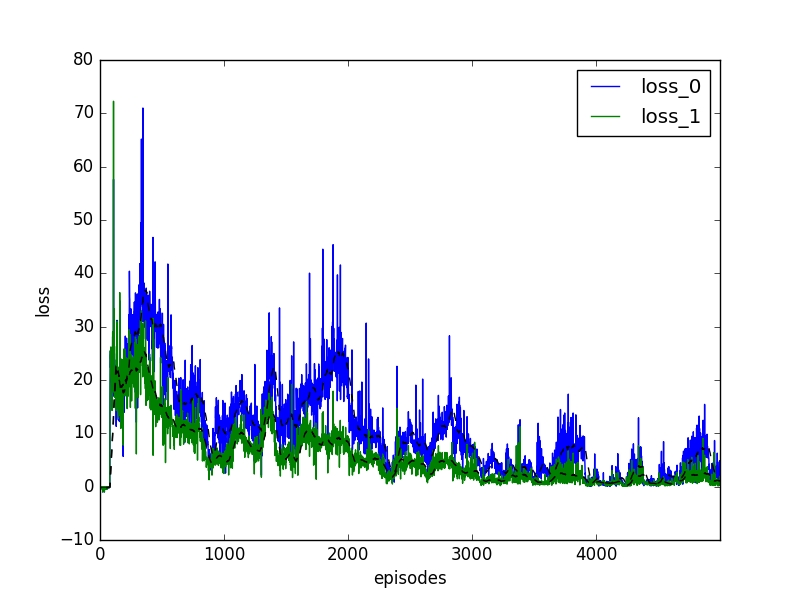
\includegraphics[width=1.5\textwidth]
    {../results/dqn_1vs1/loss.png}
    \label{fig:dqn-1vs1-loss}
  \end{subfigure}
  ~
  \begin{subfigure}[t]{\figscale\linewidth}
    \hspace*{-1.4cm}
    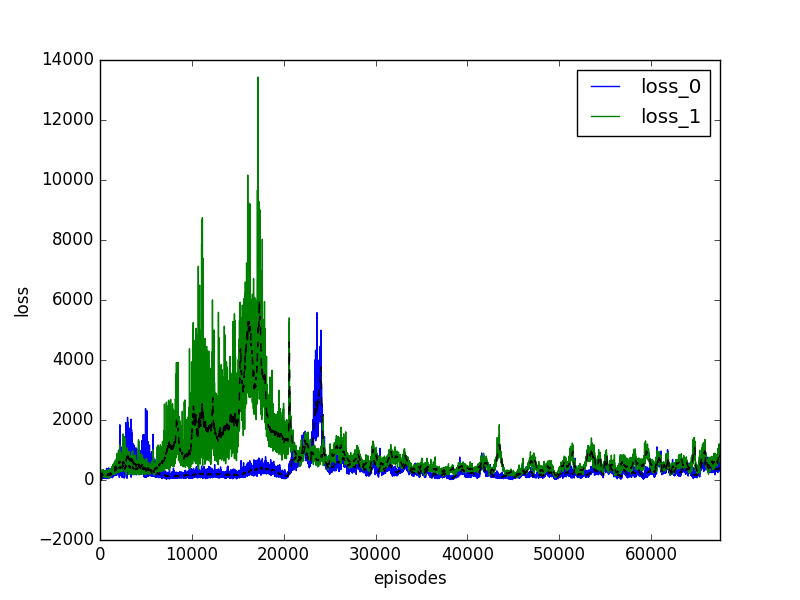
\includegraphics[width=1.5\textwidth]
    {../results/ddpg_1vs1/loss.png}
    \label{fig:ddpg-1vs1-loss}
  \end{subfigure}
  ~
  \begin{subfigure}[t]{\figscale\linewidth}
    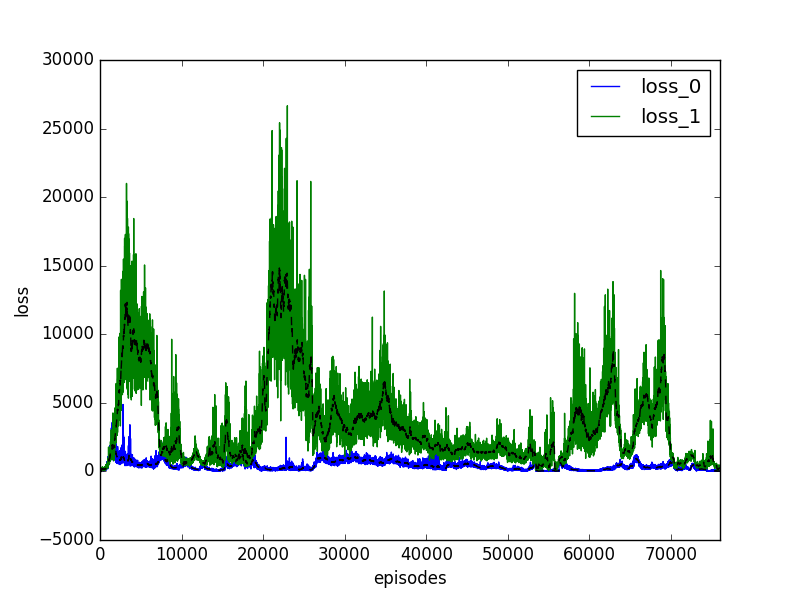
\includegraphics[width=1.5\textwidth]
    {../results/maddpg_1vs1/loss.png}
    \label{fig:maddpg-1vs1-loss}
  \end{subfigure}

  \caption{Plots for steps, average reward, collisions and loss per episode for 1 green vs 1 red agent. \textit{Left Column}: DQN, \textit{Middle Column}: DDPG, \textit{Right Column}: MADDPG}
  \label{fig:1vs1}
\end{figure}
\FloatBarrier

\subsection{2 Green Agents vs. 1 Red Agent}
\label{sec:experiment:1vs2}

\begin{figure}[t]
  \vspace*{-2cm}
  \begin{subfigure}[t]{\figscale\linewidth}
    \hspace*{-2.75cm}
    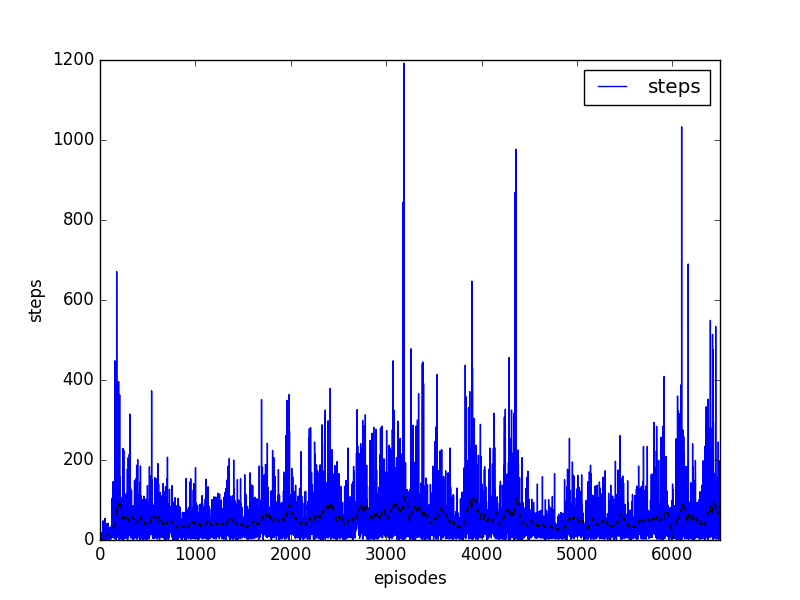
\includegraphics[width=1.5\textwidth]
    {../results/dqn_1vs2/steps.png}
    \label{fig:dqn-1vs2-steps}
  \end{subfigure}
  ~
  \begin{subfigure}[t]{\figscale\linewidth}
    \hspace*{-1.4cm}
    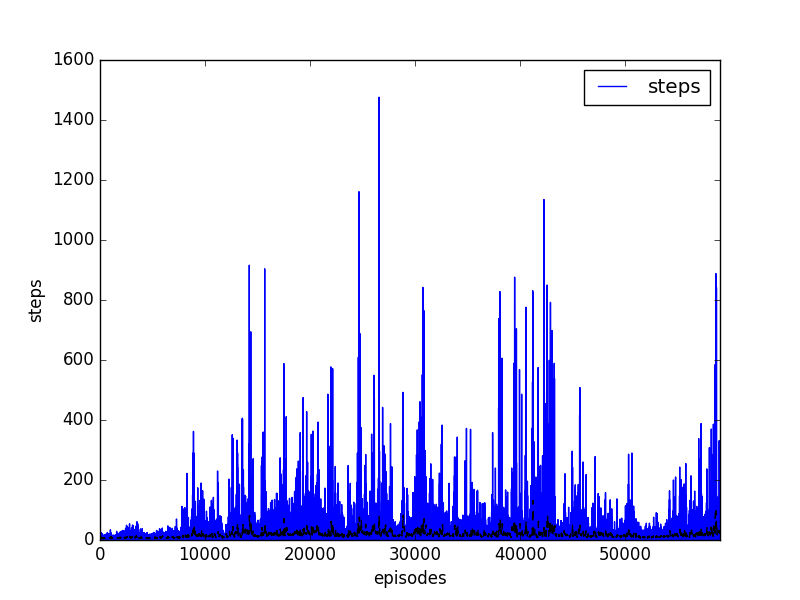
\includegraphics[width=1.5\textwidth]
    {../results/ddpg_1vs2/steps.png}
    \label{fig:ddpg-1vs2-steps}
  \end{subfigure}
  ~
  \begin{subfigure}[t]{\figscale\linewidth}
    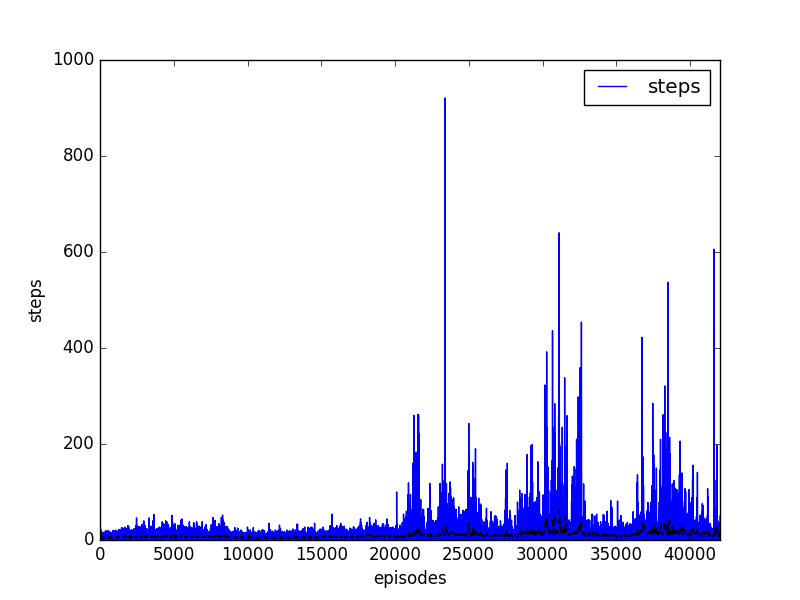
\includegraphics[width=1.5\textwidth]
    {../results/maddpg_1vs2/steps.png}
    \label{fig:maddpg-1vs2-steps}
  \end{subfigure}

  \vspace{-0.5cm}
  \begin{subfigure}[t]{\figscale\linewidth}
    \hspace*{-2.75cm}
    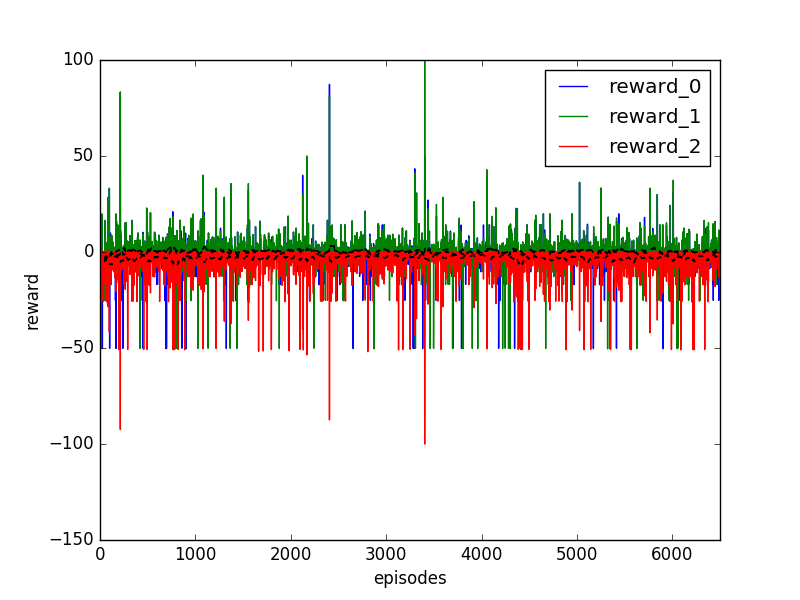
\includegraphics[width=1.5\textwidth]
    {../results/dqn_1vs2/reward.png}
    \label{fig:dqn-1vs2-reward}
  \end{subfigure}
  ~
  \begin{subfigure}[t]{\figscale\linewidth}
    \hspace*{-1.4cm}
    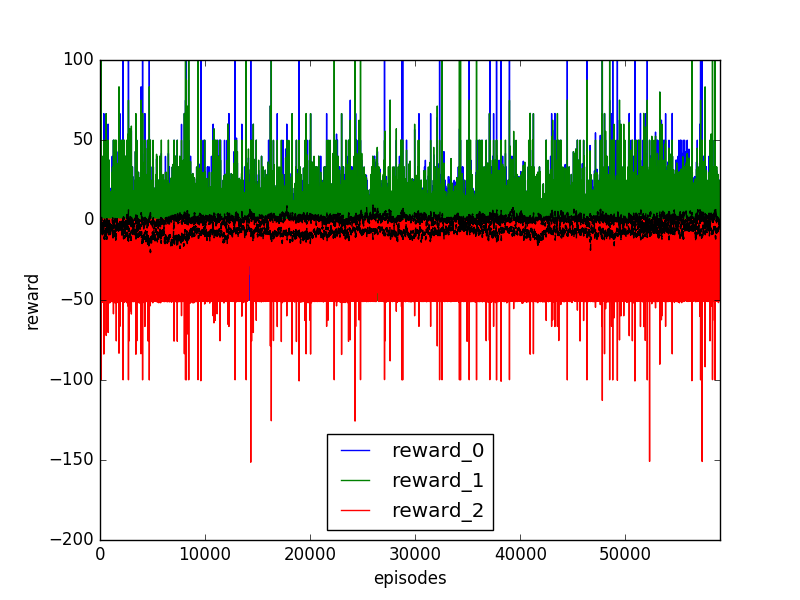
\includegraphics[width=1.5\textwidth]
    {../results/ddpg_1vs2/reward.png}
    \label{fig:ddpg-1vs2-reward}
  \end{subfigure}
  ~
  \begin{subfigure}[t]{\figscale\linewidth}
    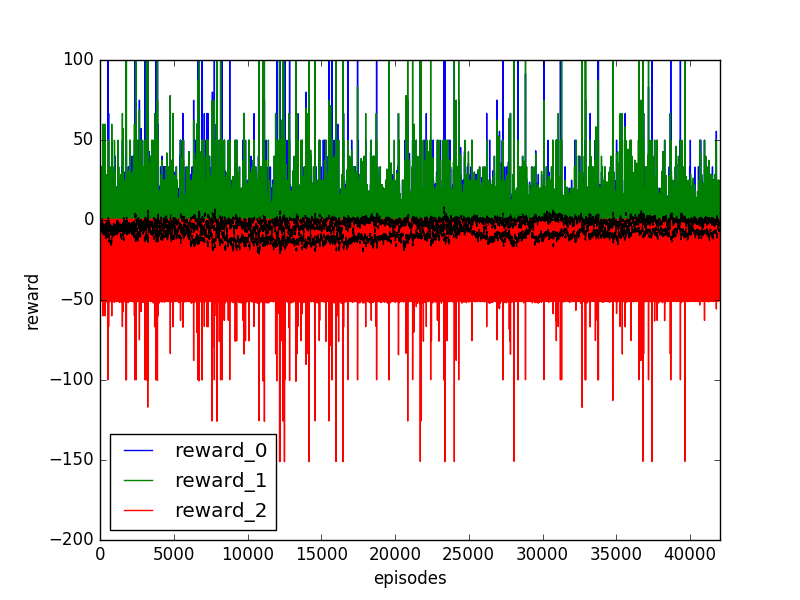
\includegraphics[width=1.5\textwidth]
    {../results/maddpg_1vs2/reward.png}
    \label{fig:maddpg-1vs2-reward}
  \end{subfigure}

  \vspace{-0.5cm}
  \begin{subfigure}[t]{\figscale\linewidth}
    \hspace*{-2.75cm}
    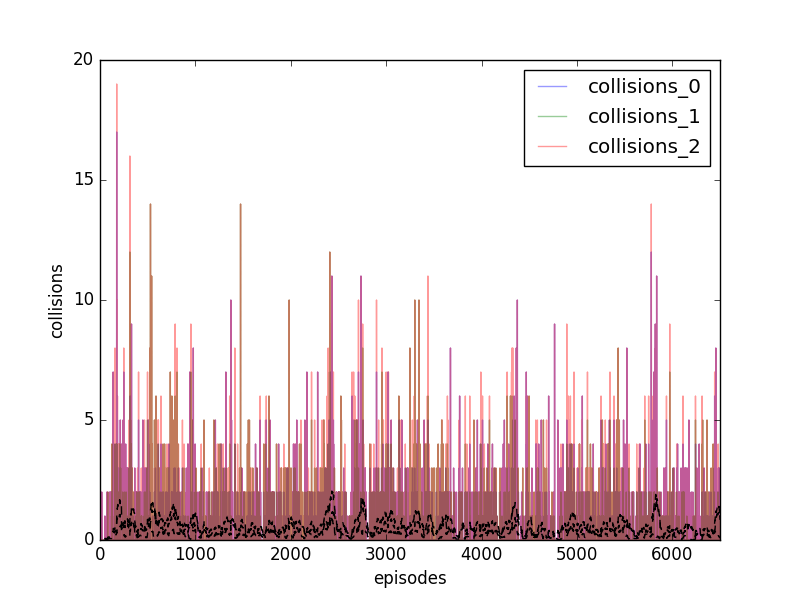
\includegraphics[width=1.5\textwidth]
    {../results/dqn_1vs2/collisions.png}
    \label{fig:dqn-1vs2-collisions}
  \end{subfigure}
  ~
  \begin{subfigure}[t]{\figscale\linewidth}
    \hspace*{-1.4cm}
    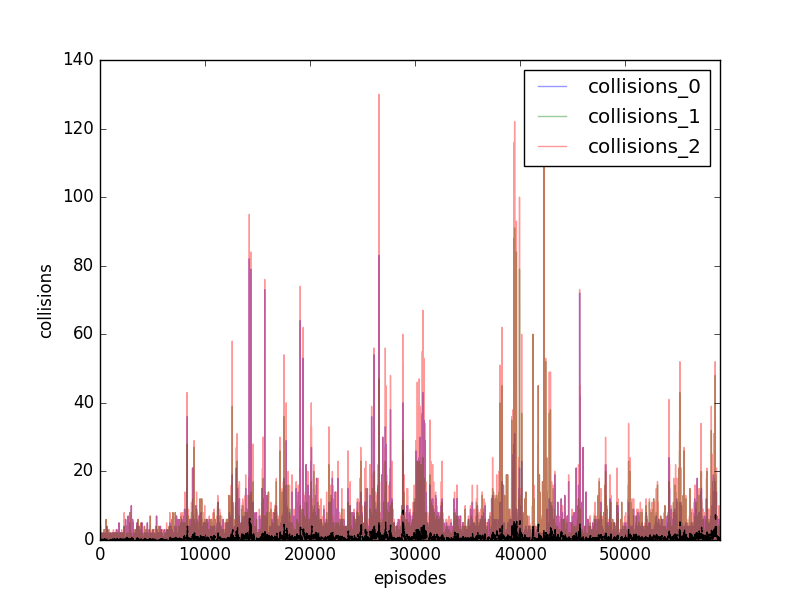
\includegraphics[width=1.5\textwidth]
    {../results/ddpg_1vs2/collisions.png}
    \label{fig:ddpg-1vs2-collisions}
  \end{subfigure}
  ~
  \begin{subfigure}[t]{\figscale\linewidth}
    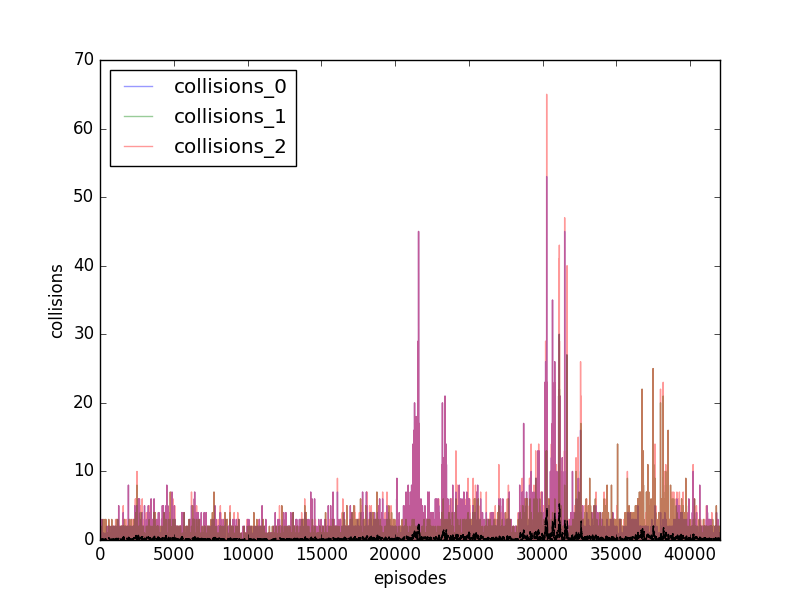
\includegraphics[width=1.5\textwidth]
    {../results/maddpg_1vs2/collisions.png}
    \label{fig:maddpg-1vs2-collisions}
  \end{subfigure}

  \vspace{-0.5cm}
  \begin{subfigure}[t]{\figscale\linewidth}
    \hspace*{-2.75cm}
    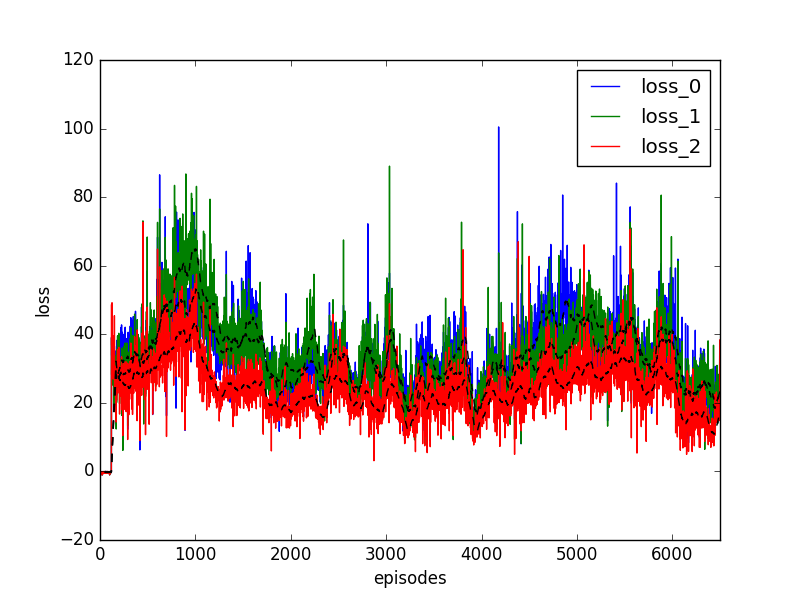
\includegraphics[width=1.5\textwidth]
    {../results/dqn_1vs2/loss.png}
    \label{fig:dqn-1vs2-loss}
  \end{subfigure}
  ~
  \begin{subfigure}[t]{\figscale\linewidth}
    \hspace*{-1.4cm}
    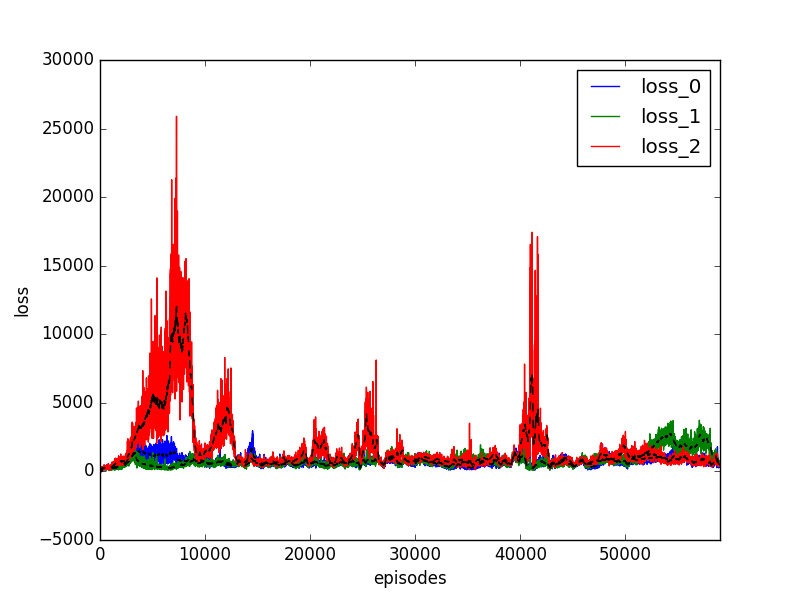
\includegraphics[width=1.5\textwidth]
    {../results/ddpg_1vs2/loss.png}
    \label{fig:ddpg-1vs2-loss}
  \end{subfigure}
  ~
  \begin{subfigure}[t]{\figscale\linewidth}
    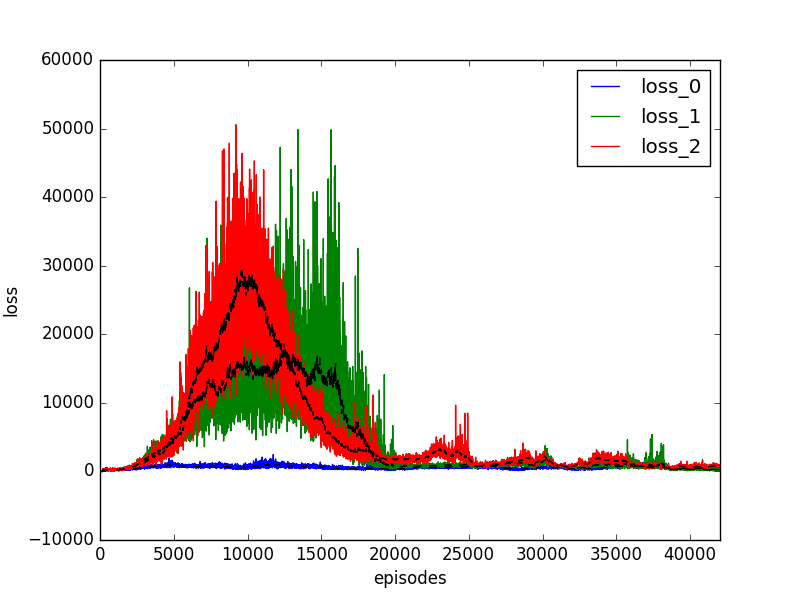
\includegraphics[width=1.5\textwidth]
    {../results/maddpg_1vs2/loss.png}
    \label{fig:maddpg-1vs2-loss}
  \end{subfigure}

  \caption{Plots for steps, average reward, collisions and loss per episode for 2 green vs 1 red agent. \textit{Left Column}: DQN, \textit{Middle Column}: DDPG, \textit{Right Column}: MADDPG}
  \label{fig:1vs2}
\end{figure}
\FloatBarrier

\subsection{1 Green Agent vs. 2 Red Agents}
\label{sec:experiment:2vs1}

\begin{figure}[t]
  \vspace*{-2cm}
  \begin{subfigure}[t]{\figscale\linewidth}
    \hspace*{-2.75cm}
    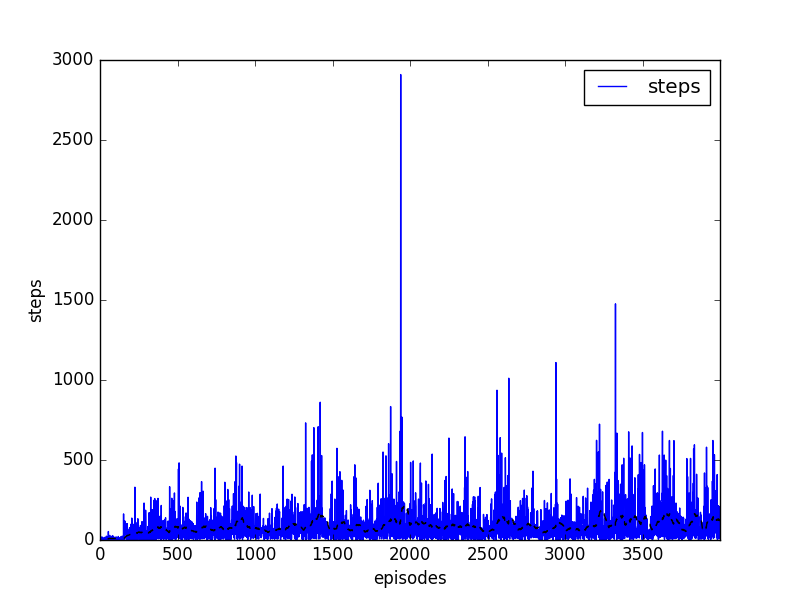
\includegraphics[width=1.5\textwidth]
    {../results/dqn_2vs1/steps.png}
    \label{fig:dqn-2vs1-steps}
  \end{subfigure}
  ~
  \begin{subfigure}[t]{\figscale\linewidth}
    \hspace*{-1.4cm}
    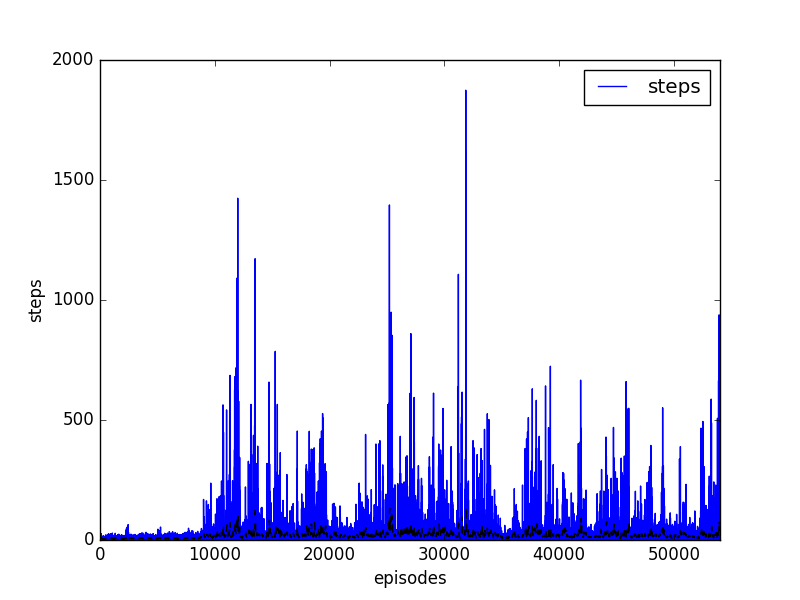
\includegraphics[width=1.5\textwidth]
    {../results/ddpg_2vs1/steps.png}
    \label{fig:ddpg-2vs1-steps}
  \end{subfigure}
  ~
  \begin{subfigure}[t]{\figscale\linewidth}
    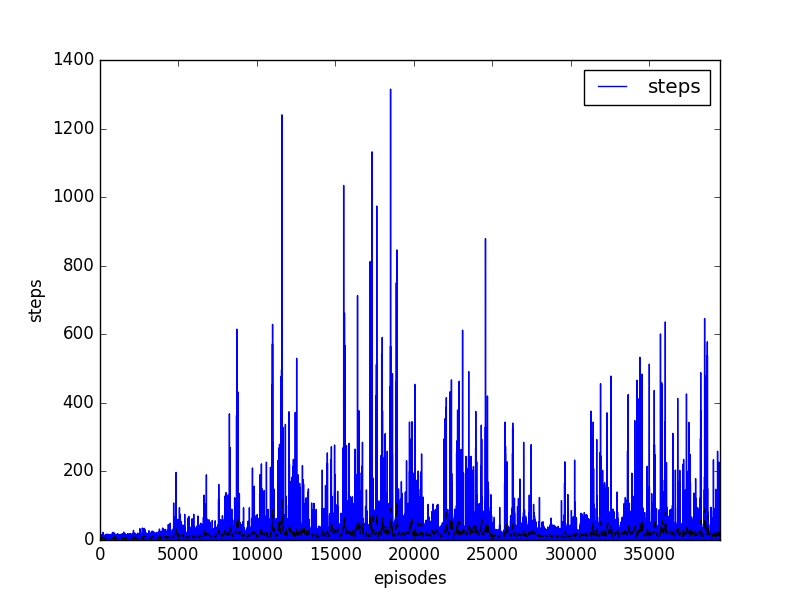
\includegraphics[width=1.5\textwidth]
    {../results/maddpg_2vs1/steps.png}
    \label{fig:maddpg-2vs1-steps}
  \end{subfigure}

  \vspace{-0.5cm}
  \begin{subfigure}[t]{\figscale\linewidth}
    \hspace*{-2.75cm}
    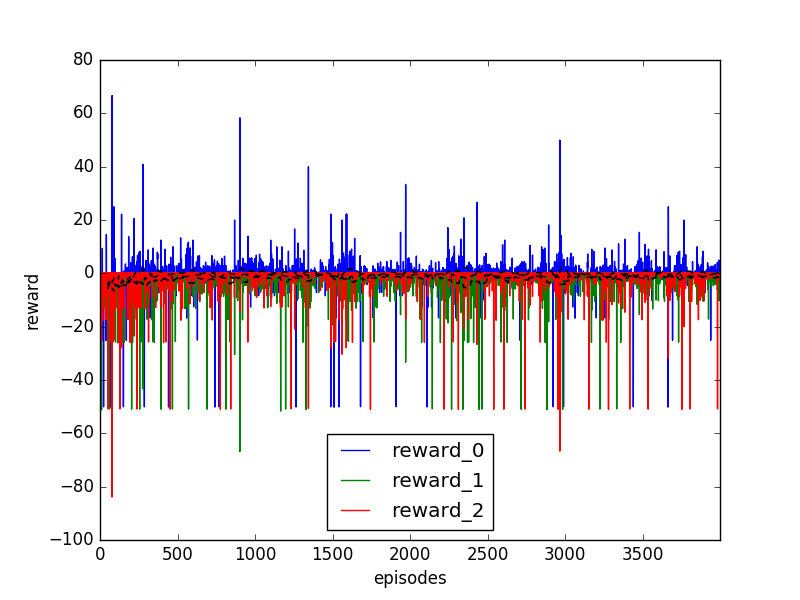
\includegraphics[width=1.5\textwidth]
    {../results/dqn_2vs1/reward.png}
    \label{fig:dqn-2vs1-reward}
  \end{subfigure}
  ~
  \begin{subfigure}[t]{\figscale\linewidth}
    \hspace*{-1.4cm}
    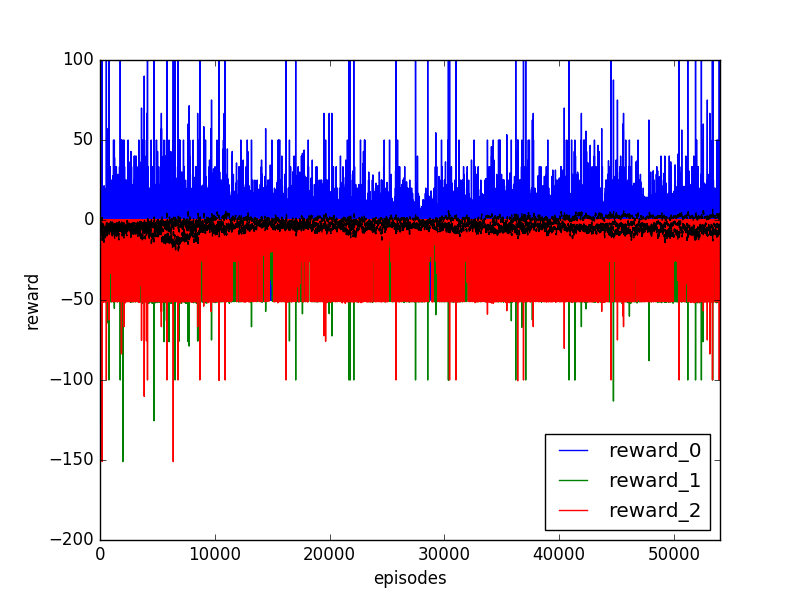
\includegraphics[width=1.5\textwidth]
    {../results/ddpg_2vs1/reward.png}
    \label{fig:ddpg-2vs1-reward}
  \end{subfigure}
  ~
  \begin{subfigure}[t]{\figscale\linewidth}
    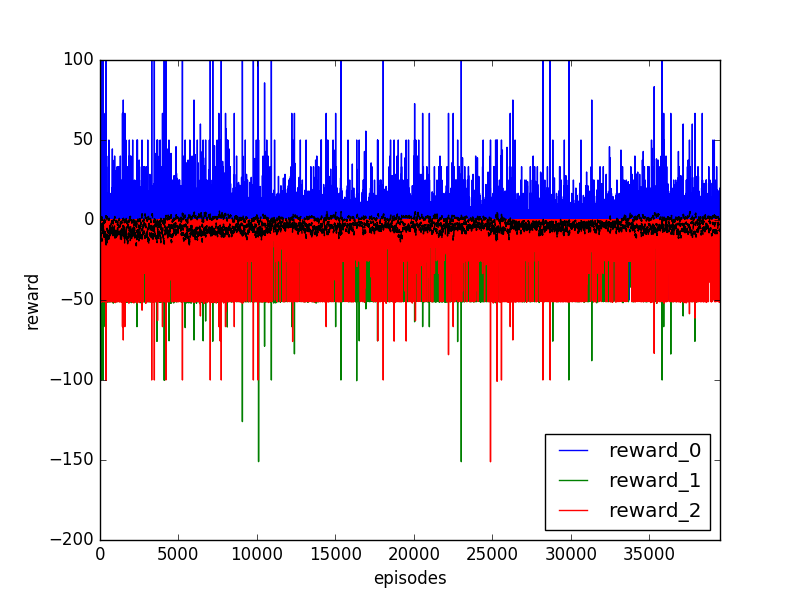
\includegraphics[width=1.5\textwidth]
    {../results/maddpg_2vs1/reward.png}
    \label{fig:maddpg-2vs1-reward}
  \end{subfigure}

  \vspace{-0.5cm}
  \begin{subfigure}[t]{\figscale\linewidth}
    \hspace*{-2.75cm}
    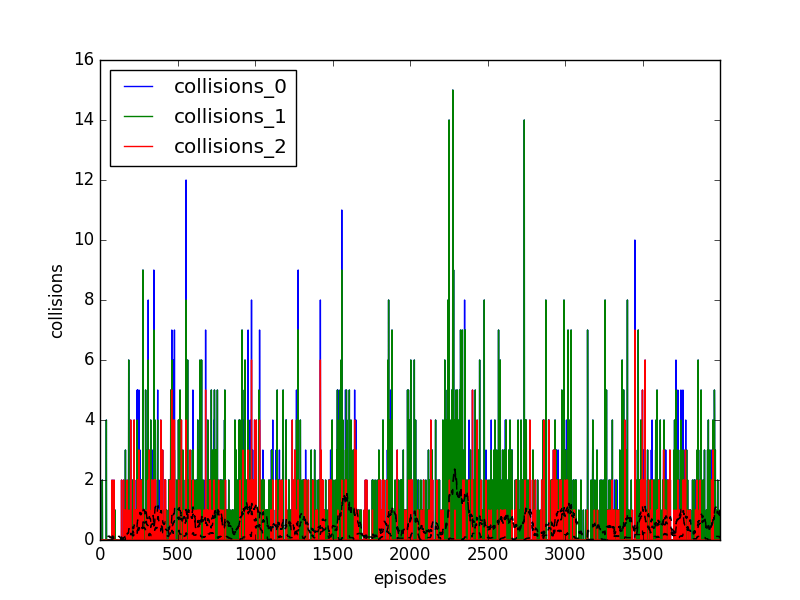
\includegraphics[width=1.5\textwidth]
    {../results/dqn_2vs1/collisions.png}
    \label{fig:dqn-2vs1-collisions}
  \end{subfigure}
  ~
  \begin{subfigure}[t]{\figscale\linewidth}
    \hspace*{-1.4cm}
    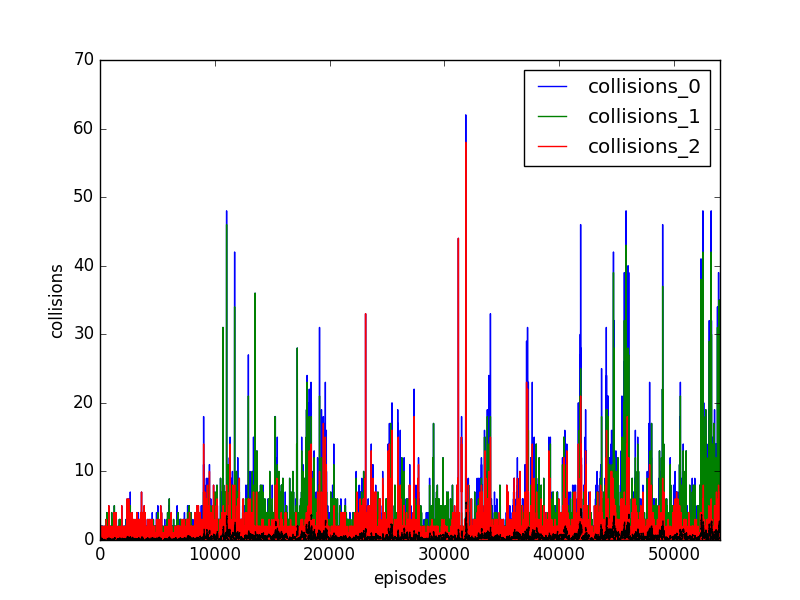
\includegraphics[width=1.5\textwidth]
    {../results/ddpg_2vs1/collisions.png}
    \label{fig:ddpg-2vs1-collisions}
  \end{subfigure}
  ~
  \begin{subfigure}[t]{\figscale\linewidth}
    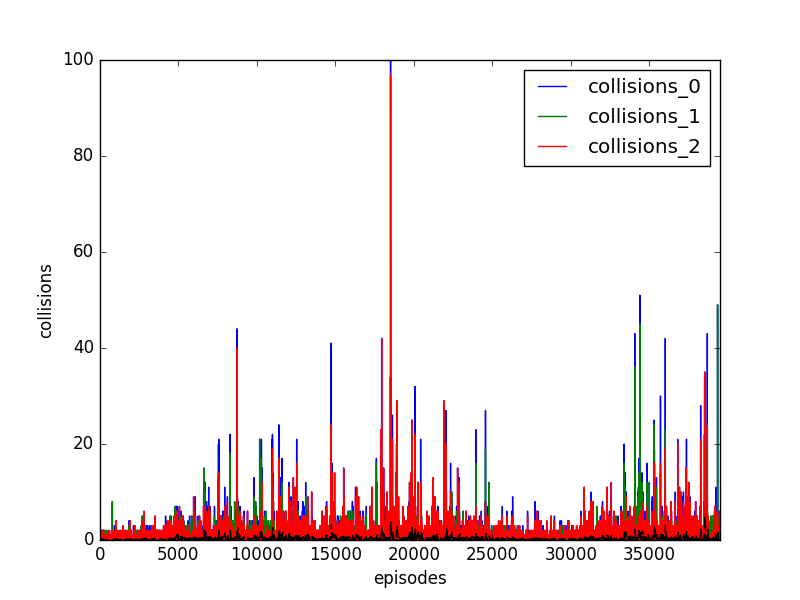
\includegraphics[width=1.5\textwidth]
    {../results/maddpg_2vs1/collisions.png}
    \label{fig:maddpg-2vs1-collisions}
  \end{subfigure}

  \vspace{-0.5cm}
  \begin{subfigure}[t]{\figscale\linewidth}
    \hspace*{-2.75cm}
    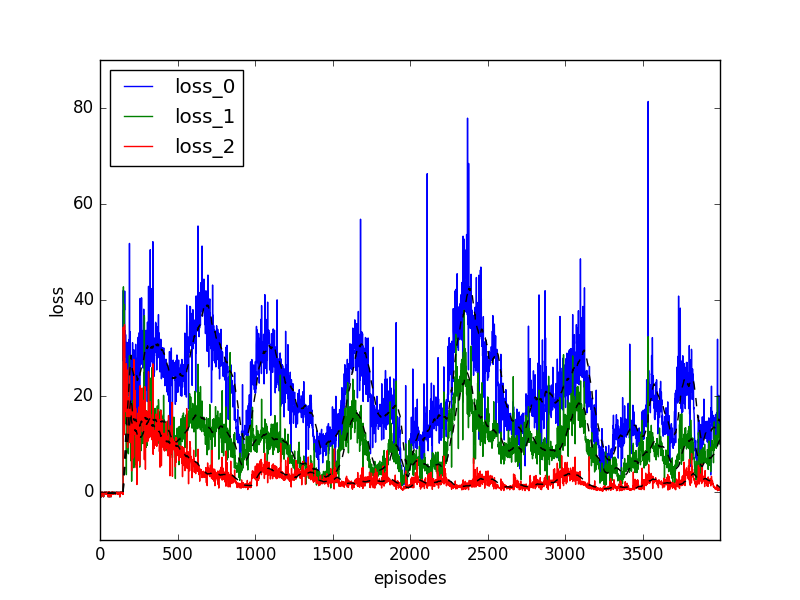
\includegraphics[width=1.5\textwidth]
    {../results/dqn_2vs1/loss.png}
    \label{fig:dqn-2vs1-loss}
  \end{subfigure}
  ~
  \begin{subfigure}[t]{\figscale\linewidth}
    \hspace*{-1.4cm}
    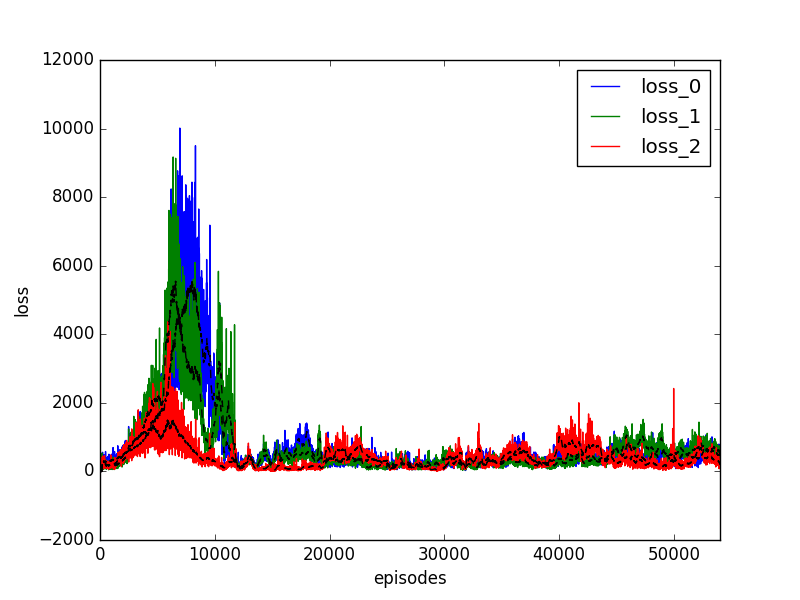
\includegraphics[width=1.5\textwidth]
    {../results/ddpg_2vs1/loss.png}
    \label{fig:ddpg-2vs1-loss}
  \end{subfigure}
  ~
  \begin{subfigure}[t]{\figscale\linewidth}
    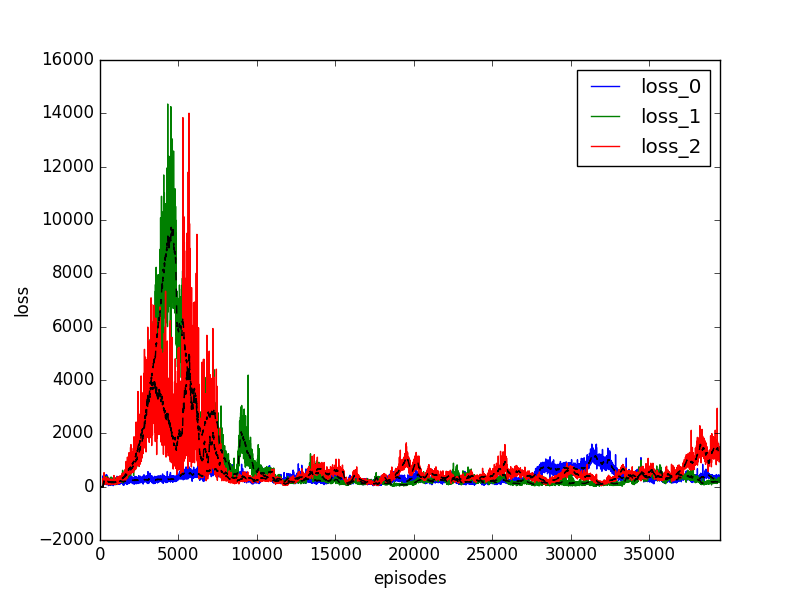
\includegraphics[width=1.5\textwidth]
    {../results/maddpg_2vs1/loss.png}
    \label{fig:maddpg-2vs1-loss}
  \end{subfigure}

  \caption{Plots for steps, average reward, collisions and loss per episode for 1 green vs 2 red agents. \textit{Left Column}: DQN, \textit{Middle Column}: DDPG, \textit{Right Column}: MADDPG}
  \label{fig:2vs1}
\end{figure}
\FloatBarrier
